\medskip

\textbf{Partie A}

\medskip

\begin{enumerate}
\item Par lecture graphique : La température initiale est $f(0) = 40$ et on observe que la température redescend à cette valeur pour $t \approx 3,8$ minutes.

\item  $f(t) = (a t + b) e^{-0{,}5t}$ donc $f(0)= (a \times 0 +b ) \times e^{0}=b$ or $f(0)=40$ donc  $b = 40$.

\item $f$ est dérivable sur $[\,0\,;\,10\,]$ comme produit de fonctions dérivables. 

$f=uv$ avec $u(t)=at+b$ et $v(t)=e^{-0{,}5t}$ donc $f'=u'v+v'u$ avec $u'(t)=a$ et $v'(t)=-0,5e^{-0{,}5t}$ 

donc pour tout $t\in [\,0\,;\,10\,]$ , $ f'(t) =  a e^{-0{,}5t} + (a t + 40)\times \left(-0{,}5e^{-0{,}5t} \right)=\left(-0{,}5 a t + a - 20\right) e^{-0{,}5t}$

donc pour tout $t\in [\,0\,;\,10\,]$ , $f'(t) + 0{,}5 f(t) = \left(-0{,}5 a t + a - 20\right) e^{-0{,}5t} + 0{,}5 (a t + 40)e^{-0{,}5t}= a e^{-0{,}5t}$

$f$ est solution de l'équation différentielle (E) donc $a e^{-0{,}5t} = 60 e^{-0{,}5t} \Rightarrow a = 60$.
\end{enumerate}

\textbf{Partie B}
 

\begin{enumerate}
\item Pour tout $t\in [\,0\,;\,10\,]$ , $ f'(t) =\left(-0{,}5 a t + a - 20\right) e^{-0{,}5t}$ avec $a=60$ on obtient $ f'(t) =(40 - 30 t) e^{-0{,}5 t}$

\item 
	\begin{enumerate}
		\item Pour tout $t\in [\,0\,;\,10\,]$ , $e^{-0{,}5t}>0$ donc $f'(t)$ a le même signe que $40 - 30t$.  

$40-30t \geqslant 0 \iff -30t \geqslant -40 \iff t \leqslant  \dfrac{4}{3}$ On en déduit le tableau de signes de $f'(t)$ et le tableau de variations de $f$ sur  $ [\,0\,;\,10\,]$ 

\begin{tikzpicture}
\tkzTabInit[lgt=3]{$y$ / 1 , Signes de $f’(t)$ / 1, Variations de $f$ / 1.5}{$0$, $\frac{4}{3}$, $10$}
\tkzTabLine{ , +, z, -, }
 \tkzTabVar{-/ $40$, +/ $120e^{-\frac{2}{3}}$, -/ $640 e^{-5}$}
\end{tikzpicture}

$f\left(\dfrac{4}{3}\right) =  \left(60 \times \dfrac{4}{3} + 40\right) e^{-0,5 \times \frac{4}{3}} = 120e^{-\frac{2}{3}}\approx 61,6$ ; $f(0)=40$ et $f(10)= 640 e^{-5} \approx 4,31 $

\item Sur $\left]\,0\,;\,\dfrac{4}{3}\,\right]$, $f(f)>40$ donc l'équation  $f(t) = 40$ n'a pas de solution. 

$\left[\,\dfrac{4}{3}\,;\,10\,\right]$ : d'après les valeurs approchées calculées dans la question précédentes, $f(\frac{4}{3}) > 40$ et $f(10) < 40$ donc $40 \in \left[\,\dfrac{4}{3}\,;\,10\,\right]$

de plus $f$ est continue ( car dérivable ) et strictement décroissante donc d'après le corollaire du théorème des valeurs intermédiaires, l'équation $f(t) = 40$ admet une unique solution $\alpha$ dans $\left[\,\dfrac{4}{3}\,;\,10\,\right]$

donc l'équation $f(t) = 40$ admet une unique solution $\alpha$
strictement positive sur $[0\,; \,10]$
`
\item À l'aide de la calculatrice on trouve $\alpha \approx 3,8$

Interprétation : La température revient à sa valeur initiale de 40~\ensuremath{^\circ} C après environ 3,8 minutes.
\end{enumerate}

\item
	\begin{enumerate}
		\item $\displaystyle \int_0^4 f(t)\,\text{d}t =\displaystyle  \int_0^4 (60 t + 40) e^{-0{,}5t} \text{d}t$.

On pose $u(t) = 60 t + 40$ et $v'(t) = e^{-0{,}5 t}$ alors $u'(t)=60$ et $v(t)= -2 e^{-0{,}5 t}$.

les fonctions $u$ et $v$ sont dérivables et leurs fonctions dérivées sont continues donc d'après la formules d'intégration par parties :

$ \displaystyle\int_0^4 (60 t + 40) e^{-0{,}5t} \text{d}t  = \left[ (60 t + 40)(-2 e^{-0{,}5t}) \right]_0^4 - \int_0^4 -2 \times 60 e^{-0{,}5t} \text{d}t = \left[(-120t -80) e^{-0{,}5t}\right]_0^4 + 120 \int_0^4 e^{-0{,}5t} \text{d}t$

$= -560e^{-2} +80 + 120 \left[-2 e^{-0{,}5t}\right]_0^4  =-560e^{-2}  +80+ 120 (-2 e^{-2} + 2)  = -560 e^{-2} + 80  -240 e^{-2} + 240$

$= 320 - 800 e^{-2} = 320 -\dfrac{800}{\mathrm{e}^{2}}$.

		\item La température moyenne de cette réaction chimique au cours des 4 premières minutes est :

$\dfrac{1}{4}\displaystyle \int_0^4 f(t)\,\text{d}t =\dfrac{1}{4} \left(320 - \dfrac{800}{e^2} \right) = 80 - \dfrac{200}{e^2} \approx  52,9$

Donc la température moyenne est environ 53~\ensuremath{^\circ} C sur les 4 premières minutes.
	\end{enumerate}
\end{enumerate}
